\documentclass[tikz,margin=5pt]{standalone}
\usepackage{tikz}
\usepackage{pgfplots}
\pgfplotsset{compat=1.16}

\usepackage{newtxtext}
\usepackage{newtxmath}
%\usepackage{mathpazo}

\usepackage{graphicx}

\begin{document}

\begin{tikzpicture}
  \node[right] at (0,0) {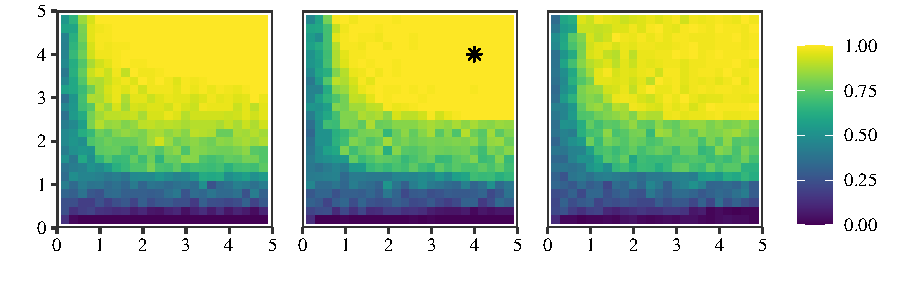
\includegraphics[scale=0.8]{../Rsession/sweep.pdf}};
  \node[right] at (-0.33,-5.0) {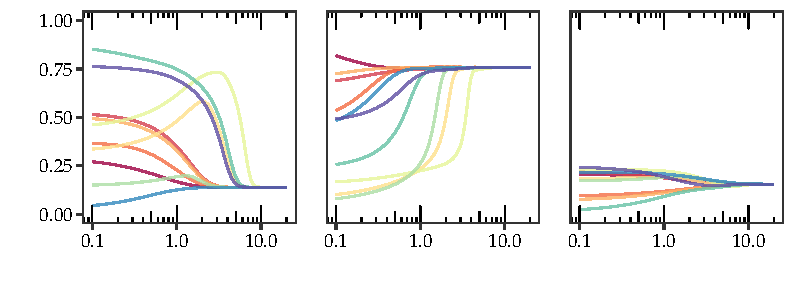
\includegraphics[scale=0.8]{../Rsession/indiv.pdf}};

  \node at (-0.5, 2.5) {\textbf{A}};
  \node at (-0.5, -2.5) {\textbf{B}};

  \node[right,align=left] at (10.80, 1.9) {\small $x_1 < \frac{1}{2} < x_2$};

  \node[left] at (0.5,0.45) {$k$};
  \node[left] at (0.2,-4.60) {$x_i(t)$};

  \node[above] at (2.35,1.9-0.12) {$\upsilon = \frac{1}{5}$};
  \node[above] at (2.35+3.33,1.9) {$\upsilon = 1$};
  \node[above] at (2.35+2*3.33,1.9) {$\upsilon = 5$};

  %\node[below] at (2.35,-1.5) {$\sigma$};
  \node[below] at (2.35+3.33,-1.5) {$\sigma$};
  %\node[below] at (2.35+2*3.33,-1.5) {$\sigma$};

  \node[above] at (2.35,-3.1) {$x_1$ (jocks)};
  \node[above] at (2.35+3.33,-3.1) {$x_2$ (burnouts)};
  \node[above] at (2.35+2*3.33,-3.1) {$x_3$ (adults)};

  %\node[below] at (2.35,-6.5) {$t$ (time)};
  \node[below] at (2.35+3.33,-6.5) {$t$ (time)};
  %\node[below] at (2.35+2*3.33,-6.5) {$t$ (time)};
\end{tikzpicture}
\end{document}

